\section{App Komponenten}
\frame{
	\frametitle{Activities}
	TODO
}

% Bild einer (Sport-)Aktivität

\frame[t]{
	\frametitle{Inversion of control}
	\begin{columns}[t]
    \column{.5\textwidth}
		\textbf{Swing}
		\begin{itemize}
			\item Classloader sucht Mainclass
			\item Classloader ruft main() auf
			\item main() erstellt JFrames nach belieben
			\item main() fügt UI Elemente hinzu
			\item main() wartet auf user input
		\end{itemize}
    \column{.5\textwidth}
	    \textbf{Android}
		\begin{itemize}
			\item Android lädt Manifest
			\item Android erstellt Activity
			\item Android ruft onCreate() auf
			\item onCreate() fügt UI Elemente hinzu
			\item Android wartet auf user input
		\end{itemize}
    \end{columns}
    %TODO Niko: als swimlane diagramm darstellen
}

\frame[c]{
	\frametitle{Activity Lifecycle}
	\begin{figure}
	\centering
	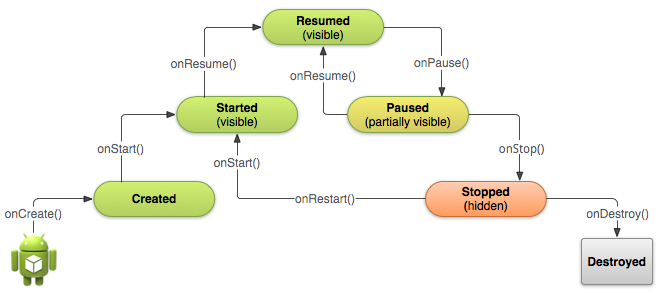
\includegraphics[width=\textwidth]{pictures/activity_lifecycle.png}
	\end{figure}
}

\frame[t]{
	\frametitle{Weitere Komponenten}
	% TODO Niko: Graphik MVC <-> Activity - Service - Content Provider + Intents + Broadcast Receiver
	\begin{itemize}
		\item View: Activity
		\item Controller: Service
		\item (Model: Content Provider)
		\item Kommunikation: Intents
		\item Listener: BroadcastReceiver
	\end{itemize}
}

\frame[t]{
	\frametitle{Intents}
	% TODO Niko: intens als kommunikationsmittel in der App und zwischen apps
}